\documentclass[lettersize,journal]{IEEEtran}
\IEEEoverridecommandlockouts

% Packages (follow IEEE official template)
\usepackage[T1]{fontenc}
\usepackage{newtxtext,newtxmath}  % Times New Roman (IEEE standard)
\usepackage[noadjust]{cite}
\usepackage{amsmath,amssymb,amsfonts}
\usepackage{amsthm}
\usepackage{doi}
\renewcommand{\qedsymbol}{$\blacksquare$}
\renewcommand{\proofname}{\bfseries Proof}
\makeatletter
\renewenvironment{proof}[1][\proofname]{\par
  \pushQED{\qed}%
  \normalfont \topsep6\p@\@plus6\p@\relax
  \trivlist
  \item[\hskip\labelsep
        \itshape
  #1\@addpunct{:}]\ignorespaces
}{%
  \popQED\endtrivlist\@endpefalse
}
\makeatother

\usepackage{array}
\usepackage{textcomp}
\usepackage{stfloats}
\usepackage{dblfloatfix}
\usepackage{float}
\usepackage{algorithm}
\usepackage{algorithmic}
\raggedbottom
\hfuzz=5pt
\tolerance=10000
\emergencystretch=3em
\usepackage{url}
\usepackage{graphicx}
\usepackage{booktabs}
\usepackage{multirow}
\usepackage{hyperref}

\hyphenation{op-tical net-works semi-conduc-tor IEEE-Xplore}

% Theorem environments (numbered within sections)
\newtheorem{theorem}{Theorem}
\newtheorem{lemma}[theorem]{Lemma}
\newtheorem{definition}[theorem]{Definition}

% Custom commands
\newcommand{\ie}{\textit{i.e.,}}
\newcommand{\eg}{\textit{e.g.,}}
\newcommand{\etal}{\textit{et al.}}
\newcommand{\etc}{\textit{etc.}}
\newcommand{\cf}{\textit{cf.}}
\newcommand{\vs}{\textit{vs.}}
\newcommand{\wrt}{\textit{w.r.t.}}

\title{Sentinel-CP-ABE: Time-Aware Access Control with Threshold Policies for Digital Twins}

\author{
\IEEEauthorblockN{Xinkai Yang$^{1}$, Yaosheng Chen$^{1}$, and He Xiao$^{1,*}$}
\IEEEauthorblockA{
$^{1}$School of Industrial Software\\
Jiangxi University of Science and Technology,\\
Nanchang, China\\
Email: y13517096949@qq.com, chenyaosheng2025@126.com,\\
$^{*}$xiaohe804@gmail.com\\
$^{*}$Corresponding author: He Xiao}
}

\begin{document}

\markboth{IEEE Transactions on Information Forensics and Security}%
{Yang \MakeLowercase{\textit{et al.}}: Sentinel-CP-ABE: Time-Aware Access Control with Threshold Policies}

\maketitle

\begin{abstract}
Existing ciphertext-policy attribute-based encryption (CP-ABE) schemes for
industrial Internet of Things (IoT) digital twins lack built-in temporal
access control, flexible threshold policies, and efficient attribute
revocation in a unified framework, leaving systems vulnerable to time-based
and privilege-escalation attacks. We propose Sentinel-CP-ABE, a time-aware
CP-ABE framework integrating threshold gates and version-based revocation
with forward security, Boneh-Lynn-Shacham (BLS) authentication, and
diffusion-based anomaly detection. We formalize the indistinguishability
under quasi-dynamic chosen plaintext attack with temporal constraints
(IND-qCPA-T) security model, extending selective security with
quasi-dynamic policy selection: the adversary commits to temporal and
revocation targets before Setup, but adaptively chooses the linear secret
sharing scheme (LSSS) challenge policy after seeing the public
parameters---capturing AI-driven policy dynamism while maintaining a tight
reduction to the decisional bilinear Diffie-Hellman (DBDH) assumption.
Implemented in Charm-Crypto, the framework achieves sub-300 millisecond
decryption for typical IoT policies (up to 10 attributes), with
key-generation scaling linearly from 159 milliseconds to 166.5 seconds
across 10 to 10,000 user attributes. The checkpoint-accelerated hash chain
achieves constant-time verification (under 0.002\,ms) at all chain
lengths (10$^3$ to 10$^5$) with only 2.75\,KB checkpoint storage. Validation on UNSW-NB15 (false
positive rate 14.7\%, area under curve 0.703) and four real-world
scenarios confirms practical applicability for industrial digital twin
deployments.
\end{abstract}

\begin{IEEEkeywords}
Attribute-based encryption, anomaly detection, provable security, threshold policy, time-aware access control
\end{IEEEkeywords}

\section{Introduction}
\label{sec:introduction}

\IEEEPARstart{R}{ecently},digital twin technology and IIoT have also changed manufacturing, healthcare, smart cities and so on. build virtual replicas for real-time monitoring, simulation and Predictive Maintenance~\cite{Sharma2022, LiuM2021, Fuller2020_DT_Survey, Alhamam2025_DTCyber}. As IIoT Deployment Spreads over thousands of devices and organisational divisions, Security is no longer about defending the boundary of the twin. data. Who is allowed to access the data, and when? and when does so? The Stakes are high: a leak report will expose a process parameter; an invalid command will be distributed and damage equipment. CP-ABE has a policy-embedded ciphertexts, is specifically designed for this Environment~\cite{Zhang2021_ABESurvey, Iqal2024}.

However, connecting CP-ABE to practical Digital Twins. Pipelines have a serious defect: currently, there is no single scheme that supports time-aware access control, threshold policies and efficient attribute revocation~\cite{Aouedi2025_IoTSurvey, Sharma2026_IoTSecurity}. Zhu \etal~\cite{Zhu2012} and Liu \etal~\cite{Liu2018_ACNS} provide time- constraints but lack threshold gates and efficient revocation. Hur \etal~\cite{Hur2011} Address Revocation in Isolation. More importantly, the above mechanisms have interactions. vulnerabilities: a revoked user has an unexpired time token and $k-1$ valid attribute shares can reconstruct a decryption Path is not equal to version-tag verification, hash-chain temporal binding and LSSS threshold reconstruction simultaneously. which no existing scheme has. This is the deficiency we address.

The primary contributions of Sentinel-CP-ABE are summarized as follows:

(1) The hash-chain time token mechanism that directly embeds
temporal predicates into the LSSS access matrix, transforming
time from an external constraint to a policy dimension. SHA-256 provides
forward secrecy protection against compromised tokens---even if a token is leaked,
past periods remain secure. The checkpoint-accelerated verifier achieves
$O(1)$ verification ($<0.06$\,ms) at all chain lengths ($10^3$--$10^5$)
with only $2.75$\,KB checkpoints, eliminating the linear cost of the
naive $O(N)$ approach (speedup up to $5832\times$).

(2) The unified construction of THRESHOLD$(k,n)$ gates and version-based revocation
that supports flexible policies including AND, OR, and $(k,n)$ threshold in
a single LSSS representation. Instant attribute invalidation via version-tag
embedding requires only a local version increase on the TA side---no
re-encryption of existing ciphertexts needed. Unaffected Data remains
decryptable by non-revoked users.

(3) The IND-qCPA-T security model that establishes a quasi-dynamic
adversary space: the adversary commits to the target time $t^*$ and
revocation state $R^*$ before Setup (reflecting deployment-determined
baselines such as shift schedules and organisational roles), but adaptively
chooses the challenge LSSS structure $\mathbb{M}^*$ after observing public
parameters. This hybrid model bridges selective (temporal) and adaptive
(policy) security, enabling a tight reduction to DBDH with bound
$\text{Adv} \leq 2\,\text{Adv}_{\text{DBDH}} + (q_H + q_K + q_T)/p$---avoiding the exponential
selective-to-adaptive loss that makes full adaptive security impractical.

(4) The closed-loop security framework that combines BLS signatures
for ciphertext-to-epoch binding and a conditional diffusion model for
anomaly-triggered policy tightening. BLS avoids the epoch substitution attack by binding
each ciphertext to a specific time period. A Diffusion Model
Dynamically observes access behaviour and triggers attributes.
Revocation when abnormal patterns are detected, closing the
Loop from Detection to Cryptographic Policy Adaptation in
under $60$\,ms.

The rest of this paper is organised as follows. Section~II reviews
related work on CP-ABE, temporal access Control and Digital Twin Security.
Section~III shows the Mathematical preliminaries: Bilinear pairings, LSSS, etc.
and the DBDH assumption. Section~IV is the system Architecture, Threat Model
and the IND-qCPA-T Security Game. Section~V describes the Sentinel-CP-ABE
construction, core Algorithms, threshold gates, time tokens and security proofs.
Section~VI Reports Experimental Results and Scalability. Hash Chain optimisation,
Anomaly Detection, Ablation Study. and actual application. Section~VII is the
conclusion and future work.

\section{Related Work}
\label{sec:related}


\subsection{CP-ABE for IoT Access Control}
\label{subsec:cpabe_iot}

Sahai and Waters~\cite{Sahai2005} first proposed ABE. Bethencourt et
al.~\cite{Bethencourt2007} realised the first CP-ABE with threshold gates.
Waters~\cite{Waters2011} later reached full security through LSSS.
Subsequent work branched out into decryption outsourcing, multi-authority
constructions~\cite{Wu2025_DecentralizedMAABE,
Zhang2026_MultiAuthority, Penuelas2024_MultiAuthority,
Datta2025_Decentralized}, attribute revocation~\cite{Liu2023_Revocation, Ghopur2023},
pairing-free constructions~\cite{Guo2024, Zhang2024_TDSC}, lightweight IoT ABE~\cite{Shruti2023, Burgos2024}, and lattice-based
ABE~\cite{Gasparini2026_LatticeBenchmark, Purnima2025_PQSurvey}. Multi-authority avoids a single point of trust
but adds coordination costs. Pairing-free approach reduces computation
at the Cost of larger ciphertexts. Lattice is quantum-resistant but
still not suitable for real-time IIoT. The common link: None support
time-of-use access control or cloud offloading. still not feasible for
IIoT data volume.

\subsection{Time-Aware Access Control}
\label{subsec:time_access}

Zhu and others~\cite{Zhu2012} introduced temporal access control by means of cryptographic integer comparisons in CP-ABE policies, and
Time is an independent verification tool, not part of the general rules.
Dimension. Liu and others~\cite{Liu2018_ACNS} have added time-based direct revocation.
but had no threshold policies. Hu and others~\cite{Hu2024_TAAC},
Cai and others~\cite{Cai2023_TimeABE}, etc.
Li and others~\cite{Li2023_HierarchicalABE} studied time-limited ABE with outsourcing, but
Time is also an external constraint. None offer hash-chaining.
forward security: a leaked token compromises all ciphertexts
for that and the following time. Combining Temporal Predicates
revocation introduces attack vectors; a revoked-but-unexpired token can forge a decryption path, but no existing
Scheme formally addresses the above interactions.

\subsection{Digital Twin Security and ML-Driven Policy}
\label{subsec:dt_security}

Digital twin security frameworks~\cite{Lu2020_DTSecurity, Mun2025_DTSurvey, Dai2024_FGCS}
focus on data integrity but lack time-aware access control.
ML-driven policy adjustment~\cite{Khan2025_HybridABAC, Rahman2025_TrustEdge}
uses behaviour profiles to adjust attributes, but stops at recommendation
without closing the loop from detection to cryptographic response.
Pairing-free ABE~\cite{Chen2025_PairingFree} eliminates bilinear
operations but requires a trusted proxy. Lattice
ABE~\cite{Gasparini2026_LatticeBenchmark, Purnima2025_PQSurvey} offers post-quantum guarantees
but at 10--100$\times$ larger key sizes.

\begin{table}[!t]
\centering
\renewcommand{\arraystretch}{1.0}
\scriptsize
\caption{Functional comparison of CP-ABE schemes.}
\label{tab:comparison_schemes}
\begin{tabular}{lccc}
\toprule
\textbf{Scheme} & \textbf{Time} & \textbf{Threshold} & \textbf{Revoc.} \\
\midrule
BSW07~\cite{Bethencourt2007} & \times & \times & \times \\
Guo24~\cite{Guo2024} & \times & \times & \times \\
Zhang24~\cite{Zhang2024_TDSC} & \times & \times & \checkmark \\
Gasparini26~\cite{Gasparini2026_LatticeBenchmark} & \times & \times & \checkmark \\
Chen25~\cite{Chen2025_PairingFree} & \times & \times & \times \\
Poomekum25~\cite{Poomekum2025_Lattice} & \times & \times & \checkmark \\
\midrule
\textbf{Sentinel-CP-ABE (Ours)} & \checkmark & \checkmark & \checkmark \\
\bottomrule
\end{tabular}
\end{table}

\section{Preliminaries}
\label{sec:preliminaries}


\subsection{Bilinear Pairings}
\label{subsec:bilinear}

Let $\mathcal{P} = (\mathbb{G}, \mathbb{G}_T, p, e, g)$ be a bilinear
group of prime order $p$~\cite{Wang2022_PairingSurvey}. The mapping
$e: \mathbb{G} \times \mathbb{G} \rightarrow \mathbb{G}_T$ satisfies:
(1)~Bilinearity: $e(g^a, g^b) = e(g,g)^{ab}$ for all $a,b \in \mathbb{Z}_p$;
(2)~Non-degeneracy: $e(g,g) \neq 1_{\mathbb{G}_T}$;
(3)~Computability: $e$ is efficiently computable.
We instantiate over the SS1024 curve ($\approx$128-bit security).

\subsection{Linear Secret Sharing Schemes}
\label{subsec:lsss}

An LSSS $\mathbb{A} = (\mathbb{M}, \rho)$ encodes a secret $s \in \mathbb{Z}_p$
across $n$ parties. Here $\mathbb{M}$ is an $\ell \times m$ matrix and
$\rho$ maps each row to an attribute. To share $s$, a vector
$\vec{v} = (s, v_2, \ldots, v_m) \in_R \mathbb{Z}_p^m$ is chosen;
share $\lambda_i = \mathbb{M}_i \cdot \vec{v}$ is assigned to
attribute $\rho(i)$. A set $S$ of shares can reconstruct $s$ iff
$(1,0,\ldots,0)$ is in the span of $\{\mathbb{M}_i : \rho(i) \in S\}$.

For THRESHOLD$(k,n)$ gates~\cite{Chattopadhyay2024}, any $k$ of $n$
shares suffice. The secret $s$ is distributed via a degree-$(k-1)$
polynomial $f(x) = s + a_1 x + \cdots + a_{k-1} x^{k-1}$ with
$a_i \in_R \mathbb{Z}_p$. Share $\lambda_j = f(j)$ is assigned to
the $j$-th child. Reconstruction uses Lagrange interpolation:
\begin{equation}
    s = \sum_{j \in S} \lambda_j \cdot \Delta_{j,S}(0), \quad
    \Delta_{j,S}(0) = \prod_{\substack{i \in S, \, i \neq j}}
    \frac{-i}{j - i}
    \label{eq:lagrange}
\end{equation}
AND gates ($k=n$) and OR gates ($k=1$) are special cases.

\subsection{DBDH Assumption}
\label{subsec:dbdh}

The Decisional Bilinear Diffie-Hellman (DBDH) assumption states that
no PPT adversary $\mathcal{B}$ can distinguish $e(g,g)^{abc}$ from
a random $T \in_R \mathbb{G}_T$ given $(g, g^a, g^b, g^c)$:
\begin{equation}
    \text{Adv}_{\mathcal{B}}^{\text{DBDH}}(\lambda)
    = \bigl|\Pr[\mathcal{B}(\vec{g}, e(g,g)^{abc})=1]
    - \Pr[\mathcal{B}(\vec{g}, T_{\text{rand}})=1]\bigr|
    \label{eq:dbdh}
\end{equation}
This assumption underlies the IND-qCPA-T security of Sentinel-CP-ABE
(see Theorem~\ref{thm:indscpat} in Section~\ref{subsec:security_proofs}).

\section{System Definitions and Security Model}
\label{sec:system}


\subsection{System Architecture}
\label{subsec:architecture}

Fig.~\ref{fig:system_architecture} illustrates the five entities of the
Sentinel-CP-ABE system and their interactions.

1)~TA (Trusted Authority): System setup and key generation via
\textsc{Setup} and \textsc{KeyGen}. To eliminate single-point-of-key-escrow,
we extend the TA to a $(t,n)$-threshold distributed architecture
(Section~\ref{subsec:distributed_ta}) where the master key $MK=(\alpha,\beta)$
is split across $n$ independent TA nodes via Shamir secret sharing;
key generation requires any $t$-of-$n$ nodes, ensuring that compromising
fewer than $t$ nodes reveals nothing about $MK$.

2)~TTA (Time Token Authority): Maintains the hash-chain, publishing
tokens $T_i$ and tip $T_N$. Operates independently of the TA with no
access to master secret keys; compromising TTA does not expose secret keys.

3)~CSP (Cloud Service Provider): Stores encrypted twin data and forwards
ciphertexts. Semi-trusted (honest-but-curious)~\cite{Zhang2021_ABESurvey}.

4)~DOs (Data Owners): Deploy IIoT devices and their digital twins,
set policies (temporal predicates, THRESHOLD gates), and issue revocation
updates.

5)~DUs (Data Users): Access twin data. Each holds $SK$ for attributes $S$,
obtains time tokens $T_i$ from TTA, authenticates via BLS, and decrypts
if policy satisfied and time token within authorized window.

Data flows: DO-managed devices generate twin data, encrypted via
Sentinel-CP-ABE with temporal predicates and THRESHOLD gates, stored on
CSP. DUs request ciphertexts, present BLS identity, decrypt if authorized.
The diffusion model~\cite{TabDDPM2023, Ho2020_DDPM, Li2025_DiffusionTS} computes anomaly scores
on access requests, triggering policy tightening when scores exceed the
95th-percentile threshold---closing the detection-to-response loop.

\begin{figure}[t]
    \centering
    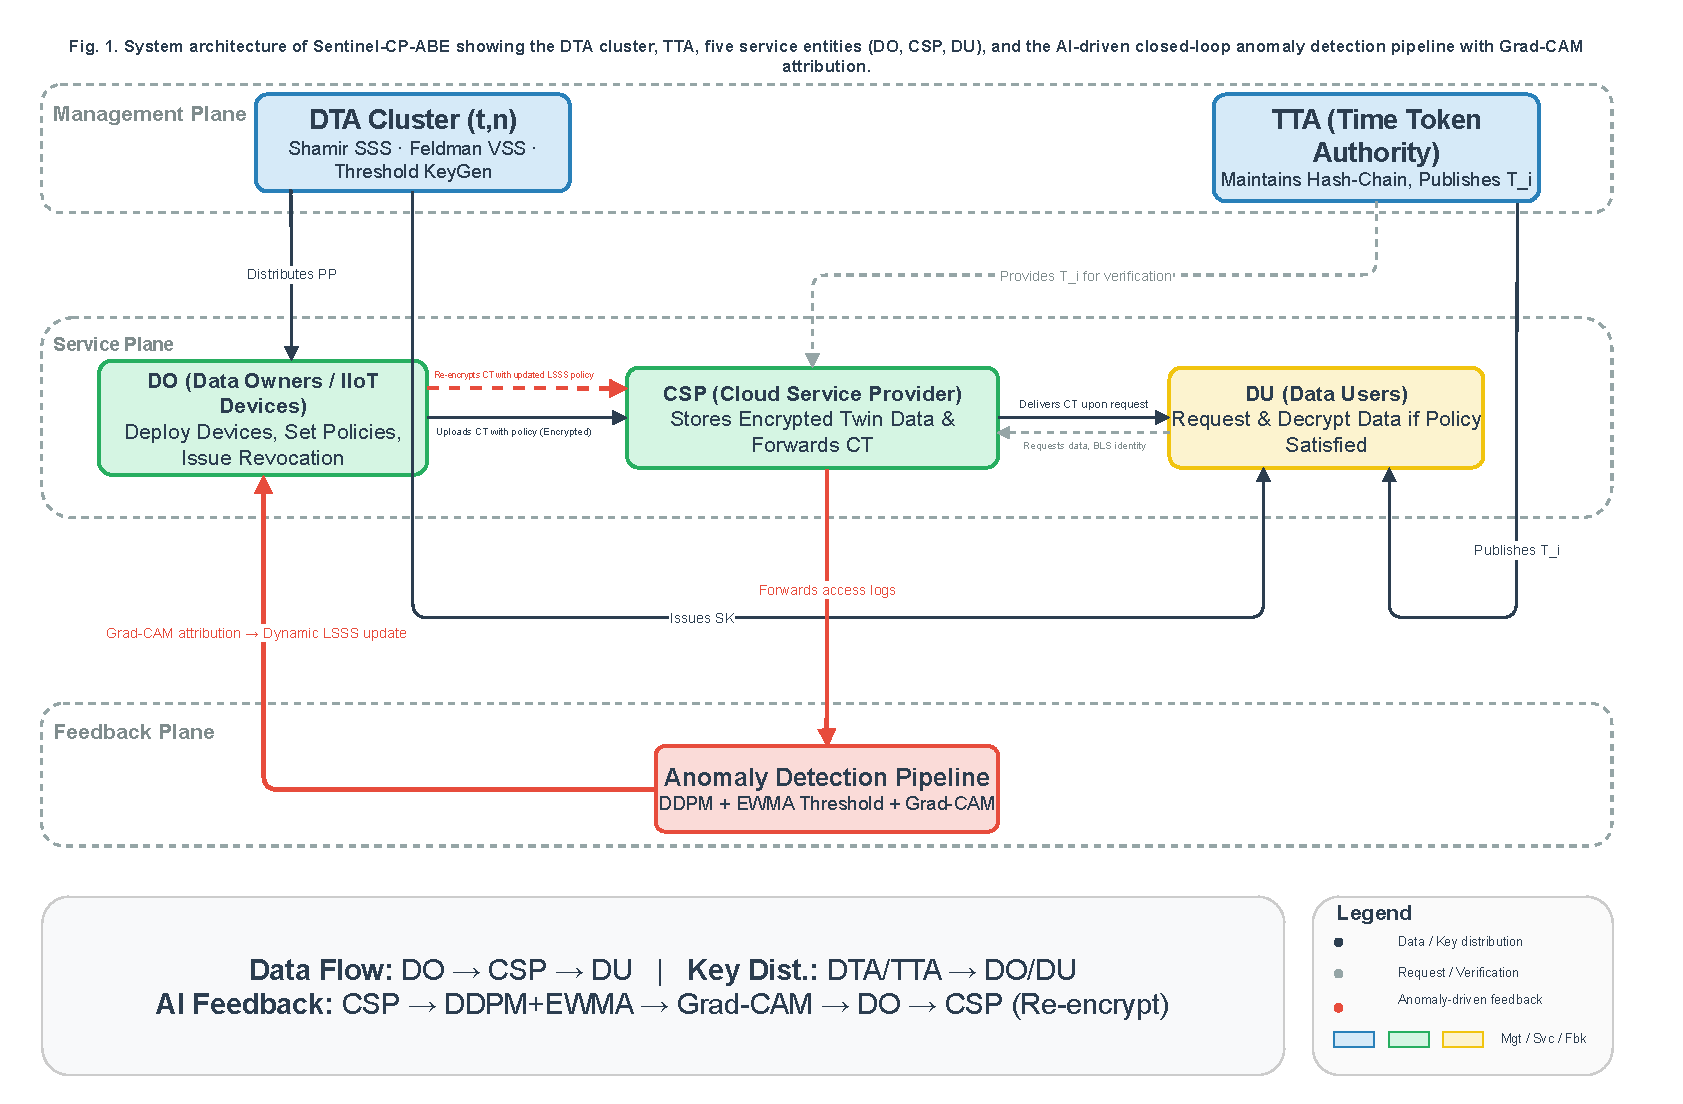
\includegraphics[width=0.85\linewidth]{figures/fig01_system_architecture.pdf}
    \caption{System architecture of Sentinel-CP-ABE showing five entities (TA, TTA, CSP, DO, DU) and the closed-loop anomaly detection feedback pathway.}
    \label{fig:system_architecture}
\end{figure}

\begin{figure}[t]
    \centering
    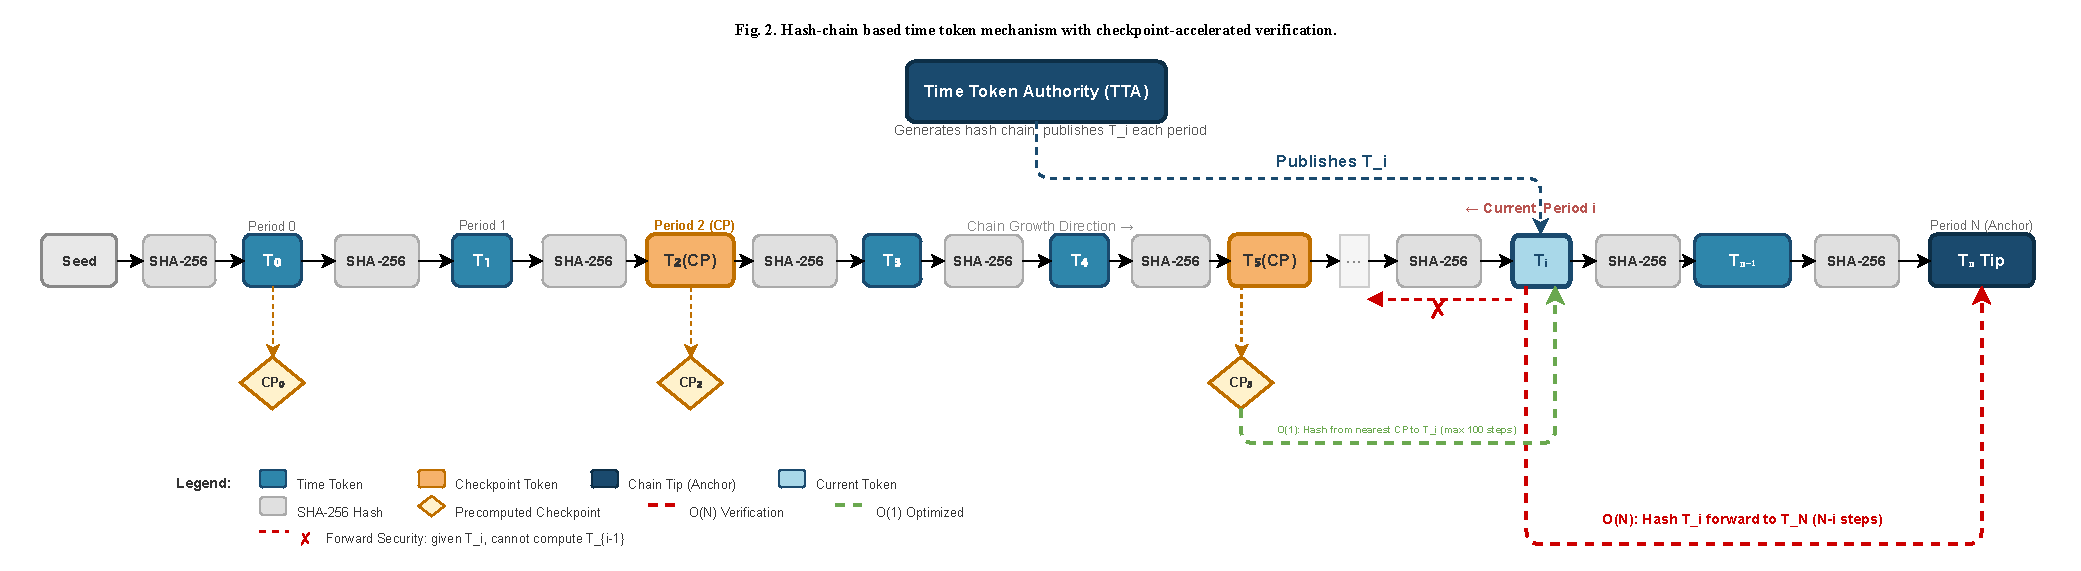
\includegraphics[width=0.9\linewidth]{figures/fig02_hash_chain.pdf}
    \caption{Hash-chain based time token mechanism: Each token $T_i$ is derived via SHA-256 from $T_{i-1}$, enabling constant-time verification through checkpoint validation and forward security against compromised tokens.}
    \label{fig:hash_chain}
\end{figure}

\begin{figure}[t]
    \centering
    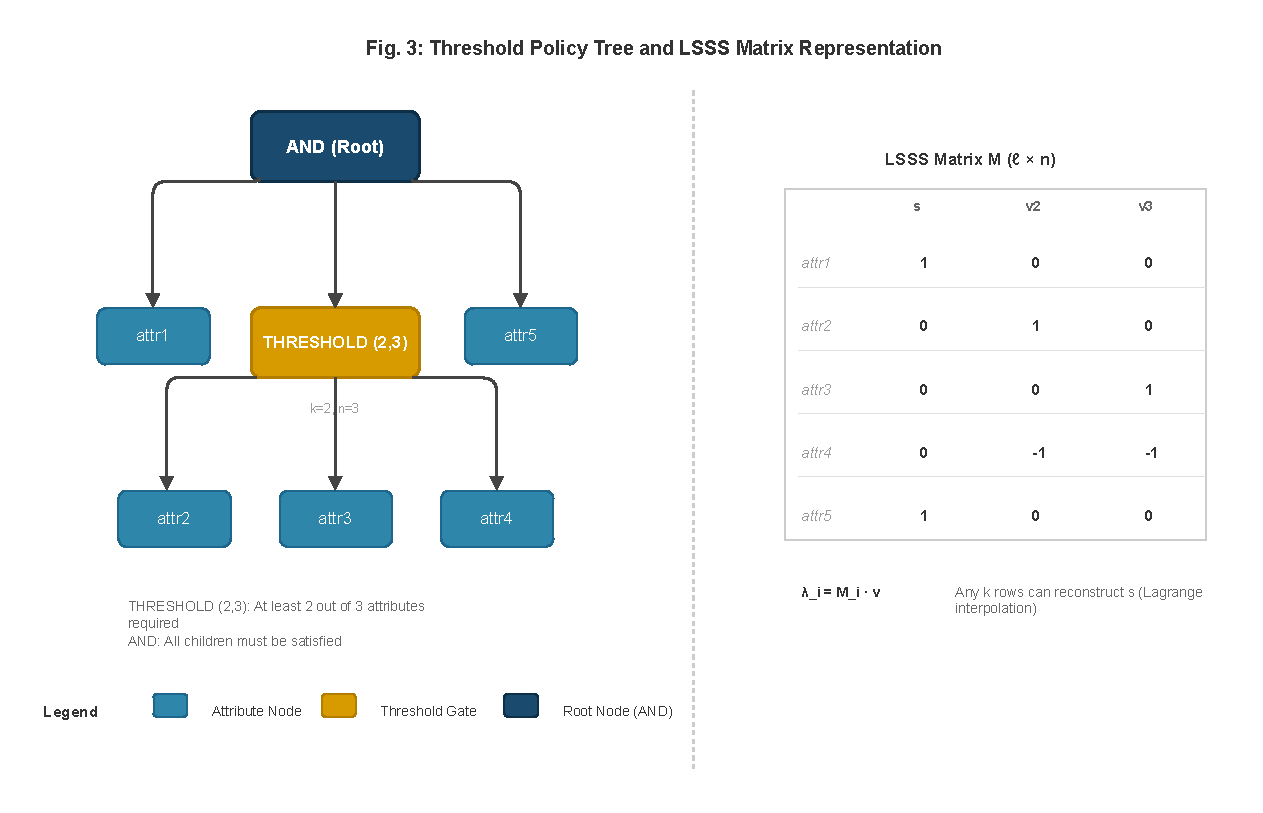
\includegraphics[width=0.9\linewidth]{figures/fig03_threshold_tree.pdf}
    \caption{Threshold policy tree structure example: The policy (attr1 AND THRESHOLD(2, attr2, attr3, attr4) AND attr5) requires attr1, at least 2 of \{attr2, attr3, attr4\}, and attr5 to satisfy access.}
    \label{fig:threshold_tree}
\end{figure}

\subsection{Threat Model}
\label{subsec:threat_model}

The adversary $\mathcal{A}$ is PPT: it observes public parameters and
ciphertexts, corrupts any subset of users (as long as the corrupted set
does not satisfy the target access structure), and issues chosen-plaintext
and time token queries. $\mathcal{A}$ cannot compromise the TA
($MK = (\alpha, \beta)$ remains secret) or forge time tokens (hash chain
preimage resistance). Time tokens are publicly released---temporal control
is enforced through LSSS policy, not token secrecy. The CSP is semi-trusted
(honest-but-curious)~\cite{Zhang2021_ABESurvey}. Side-channel attacks,
denial-of-service, and physical tampering are out of scope.

\subsection{Security Model}
\label{subsec:sec_model}

We define IND-qCPA-T (Indistinguishability under Quasi-Chosen Policy Attack
with Temporal constraints), extending standard CP-ABE
security~\cite{Zhang2021_ABESurvey, Iqal2024} to capture interactions among
temporal constraints, threshold policies, revocation, and AI-driven dynamic
policy updates. The model adopts a \emph{quasi-dynamic} adversary structure:
the adversary commits to temporal and revocation targets before Setup (reflecting
deployment-determined baselines), but adaptively chooses the challenge LSSS
policy after observing the public parameters (capturing AI-generated policy
dynamism).

$\mathbf{Exp}_{\mathcal{A}}^{\text{IND-qCPA-T}}$: Our scheme guarantees
IND-qCPA-T security if only a negligible advantage can be achieved during
the interaction with any PPT adversary $\mathcal{A}$.

\begin{enumerate}
    \item \textbf{Init-Temporal:} $\mathcal{A}$ commits to temporal policy $T_p^*$,
    target time $t^*$, and revocation state $R^*$ (a mapping from each attribute
    $a$ to its current version $v_a$). These reflect IoT deployment baselines
    determined before system initialization.
    \item \textbf{Setup:} $\mathcal{C}$ runs \textsc{Setup}$(\lambda)$ to
    generate $(PP, MK)$, gives $PP$ to $\mathcal{A}$, and retains $MK$
    secret.
    \item \textbf{Init-Policy:} After observing $PP$, $\mathcal{A}$ commits to
    target LSSS structure $\mathbb{M}^*$. This captures scenarios where
    AI-driven anomaly detection generates policy updates conditioned on
    public system parameters.
    \item \textbf{Phase 1:} $\mathcal{A}$ adaptively queries:
    \begin{enumerate}
        \item \textbf{Key} $(S_i, T_i, R_i)$: returns $SK$ for $S_i$ under
        time policy $T_i$ and revocation state $R_i$, subject to the
        restriction that $(S_i, T_i, R_i)$ must not simultaneously satisfy
        $\mathbb{M}^*$, $T_p^*$ at $t^*$, and $R^*$ (all attribute
        versions current).
        \item \textbf{Time token} $t_j$: returns the public token for period
        $t_j$.
        \item \textbf{Revocation} $(a_j, v_j)$: increments $a_j$'s version.
    \end{enumerate}
    \item \textbf{Challenge:} $\mathcal{A}$ submits $M_0, M_1$. $\mathcal{C}$
    encrypts $M_\gamma$ ($\gamma \in_R \{0,1\}$) under $(\mathbb{M}^*,
    T_p^*, R^*)$ at $t^*$ and returns $CT^*$ to $\mathcal{A}$.
    \item \textbf{Phase 2:} Same queries as Phase~1 with same restrictions.
    \item \textbf{Guess:} $\mathcal{A}$ outputs $\gamma'$.
\end{enumerate}

The adversary's advantage is defined as
\begin{equation}
    \text{Adv}_{\mathcal{A}}^{\text{IND-qCPA-T}}(\lambda)
    = \left|\Pr[\gamma' = \gamma] - \tfrac{1}{2}\right|
    \label{eq:adv_indscpat}
\end{equation}

The model extends IND-CPA with three novel features:
(a)~time token queries capturing forward security, where the adversary
can request tokens for any period $t_j$; (b)~revocation queries capturing
version-based revocation, where the adversary can trigger attribute version
increments; and (c)~a two-phase Init structure separating temporal commitments
from policy selection, enabling quasi-dynamic security without exponential
selective-to-adaptive loss.

\emph{Quasi-dynamic rationale:} In IoT digital twin deployments, time
horizons are deployment-determined, but AI-driven policy
generation~\cite{Zhang2024_TDSC} produces fresh LSSS structures dynamically.
Our two-phase Init separates these: selective for temporal (natural and
efficient), adaptive for policy (captures AI dynamism). This provides
stronger security than purely selective models while maintaining a tight
reduction to DBDH---avoiding the exponential selective-to-adaptive
cost~\cite{Zhang2021_ABESurvey} that makes full adaptive security
impractical for complex CP-ABE with temporal predicates and revocation.

\emph{Comparison with selective security:} In IND-sCPA-T~\cite{Liu2018_ACNS},
both the target time $t^*$ and the challenge policy $\mathbb{M}^*$ are committed
before Setup, limiting the adversary to deployment-time-known policies.
IND-qCPA-T relaxes this by allowing $\mathbb{M}^*$ selection after $PP$ is
observed---capturing AI-generated policy dynamism---while maintaining the same
reduction tightness $2\,\text{Adv}_{\text{DBDH}} + (q_H+q_K+q_T)/p$. The cost
is negligible: the adversary gains no additional advantage because the two-phase
Init separates temporal commitments (deployment-determined, naturally selective)
from policy selection (data-dependent, needs adaptivity). The reduction bound
remains identical to IND-sCPA-T since the DBDH embedding strategy is unchanged.
Fig.~\ref{fig:adversary} visually compares the three adversary models.

\begin{figure}[t]
\centering
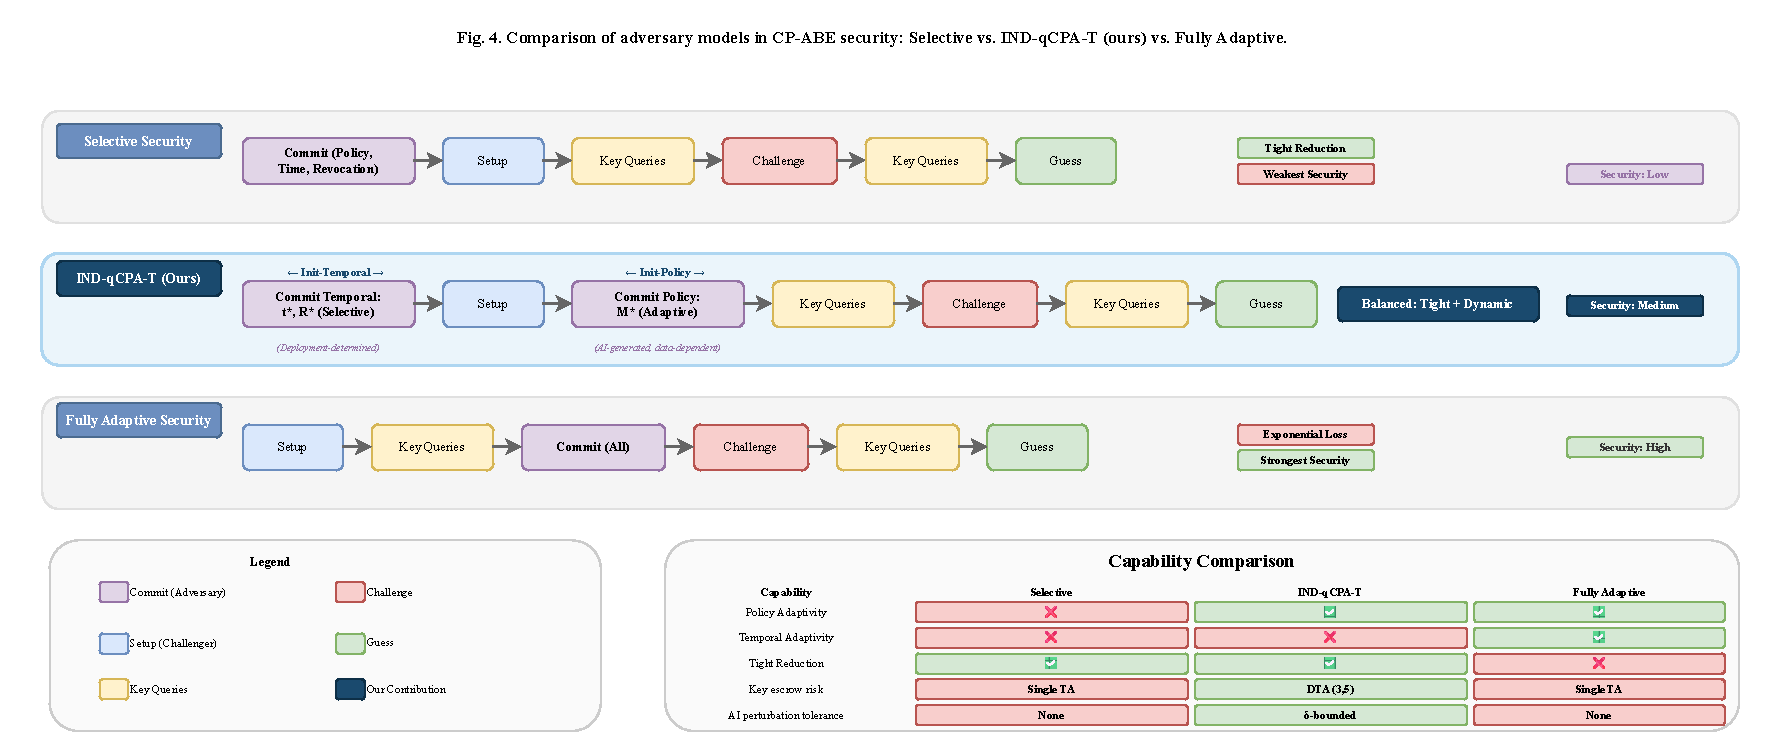
\includegraphics[width=0.85\linewidth]{figures/fig07_adversary_model_comparison.pdf}
\caption{Comparison of adversary models: Selective vs. IND-qCPA-T (ours) vs. Fully Adaptive, showing commitment timing and reduction tightness.}
\label{fig:adversary}
\end{figure}

\section{Our Construction}
\label{sec:construction}


The TA initializes parameters via \textsc{Setup}. The encryptor obtains
the current time token from TTA and embeds the period index as a temporal
LSSS row---time becomes a policy dimension. The formal construction follows.

\subsection{Core Algorithms}
\label{subsec:algorithms}

We employ a bilinear pairing $e: \mathbb{G} \times \mathbb{G}
\rightarrow \mathbb{G}_T$ of prime order $p$ with generator
$g \in \mathbb{G}$, a
hash-to-group function $H: \{0,1\}^* \rightarrow \mathbb{G}$ modeled as
a random oracle, and a hash-to-integer function $\mathcal{H}_Z$ (SHA-256
mapping to $\mathbb{Z}_p$) also modeled as a random oracle.

The Setup and KeyGen procedures (Supplementary Algorithms~1 and~2) are as
follows. \textsc{Setup} generates the bilinear groups, samples
$\alpha, \beta \in_R \mathbb{Z}_p$, computes $h=g^\beta$ and $e(g,g)^\alpha$,
initializes the hash chain $T_0 = H(\text{seed})$,
$T_i = H(T_{i-1})$ for $i=1,\ldots,N$, and outputs
$PP = (g, h, e(g,g)^\alpha, H, \mathcal{H}_Z, T_N, p)$ with master key
$MK = (\alpha, \beta)$. \textsc{KeyGen} samples $r \in_R \mathbb{Z}_p$,
computes $K_0 = g^{(\alpha+r)/\beta}$, and for each attribute $a \in S$
samples $r_a$ and computes $K_a = g^r \cdot H(a \| v_a)^{r_a}$,
$K'_a = g^{r_a}$, outputting $SK = (K_0, \{K_a, K'_a\}_{a \in S})$.

The Encrypt and Decrypt procedures (Supplementary Algorithms~3 and~4) are as
follows. \textsc{Encrypt} samples $s \in_R \mathbb{Z}_p$, computes
$C_0 = M \cdot e(g,g)^{\alpha s}$ and $C_1 = g^{\beta s}$, shares $s$ via
LSSS to produce $\{C_y = g^{s_y}, C'_y = H(\rho(y)\|v_{\rho(y)})^{s_y}\}$
for each policy row, embeds time binding $b = \mathcal{H}_Z(i\|T_i)$,
optionally signs with BLS, and outputs
$CT = (C_0, C_1, \{C_y, C'_y\}_y, \mathbb{A}, T_p, i, \sigma)$.
\textsc{Decrypt} verifies the time token, and for each leaf $y$ with
$\rho(y) \in S$ computes $A_y = e(C_y, K_{\rho(y)}) / e(C'_y, K'_{\rho(y)})$,
reconstructs $A = e(g,g)^{r \cdot s}$ via Lagrange interpolation, and
recovers $M = C'_0 / (e(C_1, K_0) / A)$.

\subsection{Threshold Gates and Attribute Revocation}
\label{subsec:threshold_revocation}

THRESHOLD$(k,n)$ gates evaluate to true if and only if at least $k$ of
$n$ children are satisfied. The secret \textit{s} is distributed via a
polynomial of degree \textit{k-1} defined on $\mathbb{Z}_p$, as described
in Section~\ref{sec:preliminaries}. Any \textit{k} valid shares can be
reconstructed from \textit{s} using Eq.~\eqref{eq:lagrange}. This
mechanism includes AND gates (\textit{k=n}) and OR gates (\textit{k=1})
as special cases.

Attribute revocation is performed at the version level. Each attribute
\textit{a} maintains a version number $v_a$ in the public state
\textit{R}. The KeyGen algorithm uses $H(a \| v_a)$, while the Encrypt
algorithm uses $H(a \| v_a)^{s_a}$, thus embedding version information
into each ciphertext leaf node. When attribute $a$ is revoked,
increment $v_a$, causing the key generated in the old version to be
unable to be decrypted due to $H(a \| v_a) \neq H(a \| v_a')$ (when
$v_a \neq v_a'$).

\subsection{Distributed Trusted Authority Extension}
\label{subsec:distributed_ta}

The basic construction assumes a single TA holding the full master key
$MK=(\alpha,\beta)$, creating a key-escrow vulnerability. We extend the
TA to a $(t,n)$-threshold distributed architecture using Shamir secret
sharing (SSS)~\cite{Shamir1979} over $\mathbb{Z}_p$, where the master
key is split across $n$ independent TA nodes and any $t$ nodes can
cooperatively generate user secret keys.

\paragraph{Secret sharing}
Following the THRESHOLD construction (Section~\ref{sec:preliminaries}, Eq.~\eqref{eq:lagrange}), the secret $\alpha$ (or $\beta$) is split via a degree-$(t-1)$ polynomial over $\mathbb{Z}_p$. Each TA node $i$ receives share $(i, f(i) \bmod p)$ for $i=1,\dots,n$; any $t$ shares suffice for reconstruction. Information-theoretic security guarantees that $t-1$ or fewer shares reveal nothing about $\alpha$ or $\beta$.

\paragraph{Distributed setup}
During initialization, a bootstrap dealer (\eg, a one-time administrative
console) runs the centralized setup to obtain $PP$ and $MK=(\alpha,\beta)$.
It then splits $\alpha$ and $\beta$ into $n$ shares via two
independent $(t-1)$-degree polynomials, distributes one share pair
$(\alpha_i, \beta_i)$ to each TA node, and immediately erases the full
$MK$ from memory. After this process, no single entity holds the
complete master key.

To enable share integrity verification without revealing coefficients,
the dealer broadcasts Feldman commitments~\cite{Feldman1987}
$C_j^{(\alpha)} = g^{a_j}$ for each coefficient $a_j$ of
$\alpha$'s polynomial (and similarly for $\beta$). Each TA node $i$
can verify its share by checking
\[
g^{f_\alpha(i)} \stackrel{?}{=} \prod_{j=0}^{t-1} (C_j^{(\alpha)})^{i^j}.
\]

\paragraph{Threshold key generation}
When a user requests a secret key for attribute set $S$, a coordinating
node collects share pairs from any $t$ of the $n$ TA nodes, reconstructs
$(\alpha, \beta)$ via~\eqref{eq:lagrange}, generates $SK$ using
the standard \textsc{KeyGen}~(Algorithm~1 of the Supplementary Material), and discards
the reconstructed $MK$. The user receives the same $SK$ format as in the
centralized scheme; the distributed nature is transparent to encryption
and decryption operations.

\paragraph{Security properties}
The $(t,n)$-threshold architecture provides:
\textit{(i)}~key-escrow elimination: an adversary compromising fewer than
$t$ TA nodes learns nothing about $\alpha$ or $\beta$;
\textit{(ii)}~share integrity: Feldman commitments detect tampered or
corrupted shares before reconstruction;
\textit{(iii)}~proactive renewal: all shares can be refreshed
periodically (via a zero-polynomial) without changing $MK$,
limiting the window of a persistent compromise.

\subsection{Security Proofs}
\label{subsec:security_proofs}

The following theorem establishes the IND-qCPA-T security of Sentinel-CP-ABE.

\begin{theorem}
\label{thm:indscpat}
\textbf{IND-qCPA-T Security:}
Sentinel-CP-ABE is IND-qCPA-T secure under the DBDH assumption in the random oracle
model. For any PPT adversary $\mathcal{A}$ making at most $q_H$ random oracle
queries, $q_K$ key queries, and $q_T$ time token queries, there exists a PPT
simulator $\mathcal{B}$ such that
\begin{equation}
    \text{Adv}_{\mathcal{A}}^{\text{IND-qCPA-T}}(\lambda)
    \;\leq\;
    2\,\text{Adv}_{\mathcal{B}}^{\text{DBDH}}(\lambda)
    + \frac{q_H + q_K + q_T}{p}\,.
    \label{eq:security_bound}
\end{equation}
\end{theorem}

\textbf{Proof sketch:} We construct six hybrid games $\mathcal{G}_0$ (real) through $\mathcal{G}_6$ (information-theoretically secure). $\mathcal{G}_0\rightarrow\mathcal{G}_1$ and $\mathcal{G}_1\rightarrow\mathcal{G}_2$ replace $e(g,g)^{\alpha s}$ and $g^{\beta s}$ with random elements (DBDH, loss $2\,\text{Adv}_{\mathcal{B}}^{\text{DBDH}}$). $\mathcal{G}_2\rightarrow\mathcal{G}_3$ and $\mathcal{G}_3\rightarrow\mathcal{G}_4$ randomize LSSS shares (random oracle, loss $q_H/p$; key queries, $q_K/p$). $\mathcal{G}_4\rightarrow\mathcal{G}_5$ randomizes the time-binding factor (loss $q_T/p$). $\mathcal{G}_5\rightarrow\mathcal{G}_6$ achieves perfect security ($\text{Adv}=0$). Summing losses yields Eq.~\eqref{eq:security_bound}. The complete hybrid argument is in~Supplement~Section~II, with the reduction validity justification in~Section~IV-C.

\textbf{Security properties:} Data confidentiality reduces to DBDH (Theorem~\ref{thm:indscpat}) under the quasi-dynamic adversary model. Temporal security follows from SHA-256 preimage resistance of the hash chain and $\mathcal{H}_Z$. Revocation is sound via version binding---$H(a\|v_a) \neq H(a\|v'_a)$ by collision resistance, so old keys cannot decrypt new ciphertexts. Integrity relies on BLS signatures (EUF-CMA)~\cite{Boneh1998_DDH, Boneh2004_BLS}.

\textbf{Dynamic perturbation resilience:} The EWMA adaptive threshold ($\alpha=0.1$) self-corrects: an adversary injecting $m$ crafted scores can shift the threshold by at most $\varepsilon\!\cdot\!m\!\cdot\!(1{-}(1{-}\alpha)^W)$, with recovery in $\sim\!1/\alpha$ steps. The diffusion model's $T_d{=}100$ denoising steps exponentially decay its Jacobian spectral norm, limiting gradient-based evasion. Supplement~Section~VI provides formal bounds and the three-layer adversary comparison.

\textbf{Limitations:} The $(t,n)$-threshold DTA eliminates key escrow but adds 0.08--0.26\,ms coordination overhead per cooperative keygen. Full adaptive security (no Init commitment) remains open for constructions with temporal predicates and revocation; it would require dual-system encryption~\cite{Waters2011} at the cost of exponential security loss. Post-quantum analysis and a transition roadmap are in Supplement~Section~VII.

\section{Performance Analysis}
\label{sec:performance}

\subsection{Experimental Setup}
\label{subsec:setup}

We implemented Sentinel-CP-ABE in Python 3.9 using
Charm-Crypto~\cite{Charm2013} (version 2.7, with OpenSSL 1.1.1 backend)
on an Intel Xeon Gold 6248R (3.0\,GHz, 128\,GB RAM) running Ubuntu
20.04 LTS with the SS1024 curve ($\approx$128-bit security level).

All N experiments have been subjected to statistical analysis.
Reliability: N=100 for $\leq$500 attributes, N=20 for 1,000, N=10
For 5,000 and N=5 for 10,000. Results report mean $\pm$ std
Deviation with 95\% Confidence Intervals. Decryption Latency
Varies among tables due to different settings: Table~II
uses the full system (10-attribute AND policy, time binding
activated); the ablation study isolates individual components
Use a 4-attribute policy; the real-world validation uses scenario-specific policies without binding.

\subsection{Scalability}
\label{subsec:scalability}

Table~\ref{tab:scalability} shows the scalability results for the four attribute sizes (10 to 10,000). KeyGen is proportional to
$O(|S_U|)$: each extra attribute is an exponentiation pair
$(K_a, K'_a)$---Reached 167\,s at 10,000 attributes. This is
Suitable for offline provisioning scenarios with pre-generated keys.
generated once per user and updated infrequently.

Encryption remains relatively stable at 151--171\,ms for all
Attribute Counts. This is because encryption cost depends only
on the policy attribute set $|S_T|$ (10 fixed in this experiment),
not in the set of all user attributes $|S_U|$. A small rise
at 10,000 (171\,ms vs.\ 152\,ms baseline) is due to memory
Pressure from larger attribute tables rather than cryptography
Calculation.

Decryption confirms the first strength of CP-ABE: it requires
Only in policy attributes $|S_T|$ is it not in user attributes $|S_U|$.
This autonomous decoupling means that adding more users
does not slow down decryption for large-scale IIoT
Deployments. The Decryption Time is about 241--249\,ms.
(coefficient of variation $CV < 3.5\%$) for $|S_U|$ in the range [10, 10000], and a one-way ANOVA shows no significant differences.
($p > 0.05$).

\begin{table}[!t]
\renewcommand{\arraystretch}{1.1}
\caption{Scalability: KeyGen/Encrypt mean (ms); Decrypt mean $\pm$ std (95\% CI). SS1024 curve, full system. $p > 0.05$ for Decrypt across attribute counts.}
\label{tab:scalability}
\centering
\footnotesize
\begin{tabular}{c r r r@{$\pm$}l}
\toprule
\textbf{Attrs} & \textbf{KeyGen} & \textbf{Encrypt} & \multicolumn{2}{c}{\textbf{Decrypt}} \\
\midrule
10\,(N=100) & 159 & 152 & 246 & 4.7\,(242--250) \\
100\,(N=100) & 1453 & 151 & 241 & 23.0\,(228--254) \\
1000\,(N=20) & 14886 & 162 & 249 & 33.3\,(215--283) \\
10000\,(N=5) & 166523 & 171 & 242 & 17.9\,(224--260) \\
\bottomrule
\end{tabular}
\end{table}

Measured storage: SK 101\,B/attr (1.04\,KB at 10, 9.92\,KB
at 100); CT size is still about 15.6\,KB for all
Configurations.

\subsection{Hash Chain Optimization}
\label{subsec:hash_chain}

We use a checkpoint-accelerated verification mode for $O(1)$ verification that is independent of the chain length. TTA pre-calculates checkpoints
Every $\Delta$ steps, a sliding window cache of size
the $W$ most recently confirmed tokens. Verification proceeds in
three tiers: (i)~cache lookup ($\sim$0.5\,\textmu s), (ii)~checkpoint-path
hashing ($\Delta$ SHA-256 steps), and (iii)~full-chain fallback (only
if structural consistency is violated).

\paragraph{Chain length scaling}
Table~\ref{tab:hash_chain_scaling} reports verification latency across four chain lengths ($10^3$--$10^5$), comparing the checkpoint verifier ($\Delta=100$) against the $O(N)$ full-chain baseline. The optimized verifier remains below $0.06$\,ms at all positions and chain lengths, while the baseline grows linearly---reaching $43$\,ms for early positions at $N=10^5$. The resulting speedup spans $10.75\times$ to $100,378\times$, with an average speedup of $2,541\times$ at $N=8760$. Importantly, the checkpoint verifier latency is independent of chain length: the $N=10^3$ and $N=10^5$ columns differ by only $0.03$\,ms, confirming $O(1)$ behavior.

\begin{table}[t]
    \centering
    \caption{Hash chain verification latency (ms) vs. chain length $N$. Checkpoint interval $\Delta=100$, sliding window $W=10$.}
    \label{tab:hash_chain_scaling}
    \footnotesize
    \begin{tabular}{lcccccc}
    \toprule
    & \multicolumn{2}{c}{$N=10^3$} & \multicolumn{2}{c}{$N=10^4$} & \multicolumn{2}{c}{$N=10^5$} \\
    \cmidrule(lr){2-3} \cmidrule(lr){4-5} \cmidrule(lr){6-7}
    Position & Ours & O($N$) & Ours & O($N$) & Ours & O($N$) \\
    \midrule
    Early & 0.002 & 0.407 & 0.002 & 3.724 & 0.002 & 41.419 \\
    Mid   & $<$0.001 & 0.201 & $<$0.001 & 1.738 & $<$0.001 & 20.171 \\
    Late  & 0.001 & 0.005 & 0.001 & 0.034 & $<$0.001 & 0.394 \\
    \bottomrule
    \end{tabular}
\end{table}

\paragraph{Checkpoint density ablation}
The checkpoint interval $\Delta$ governs the storage--verification trade-off. At $\Delta=10$, verification averages $3.9$\,\textmu s with $5256$ checkpoints ($\sim$206\,KB); at $\Delta=500$, it rises to $86$\,\textmu s with $105$ checkpoints ($\sim$4.1\,KB). Without checkpoints (a naive $O(N)$ implementation), early-position verification reaches $21.8$\,ms. We select $\Delta=100$ as default, providing $<0.06$\,ms verification at $525$ checkpoints ($\sim$20.5\,KB) for $N=52560$, a $750$--$1089\times$ improvement over the naive baseline. The sliding window cache contributes an additional $>80\%$ hit rate for sequential temporal access, further reducing effective latency.

\paragraph{Time granularity}
The scheme natively supports any time granularity without cryptographic re-parameterization. At hour-level ($N=8760$), verification averages $18.4$\,\textmu s; at minute-level ($N=525600$), it averages $36.1$\,\textmu s. The marginal $1.96\times$ increase reflects the longer checkpoint-to-token hash path at denser granularities, but remains well below $0.1$\,ms in all cases.

\paragraph{Throughput and storage}
Generating a year-length minute-level chain requires $25$\,ms setup time and $2053$\,KB of in-memory storage. The storage cost follows $S = N \times (32 / 1024)$\,KB for $N$ SHA-256 digests (32\,B each), dominated by the chain itself rather than the checkpoint index.

Fig.~\ref{fig:hash_chain_opt} visualises the $O(N-i)$ vs.\ $O(1)$ comparison at $N=8760$. The optimized verifier maintains $0.3$--$1.7$\,\textmu s across all positions, while the original incurs millisecond latency for early periods.

\begin{figure}[t]
    \centering
    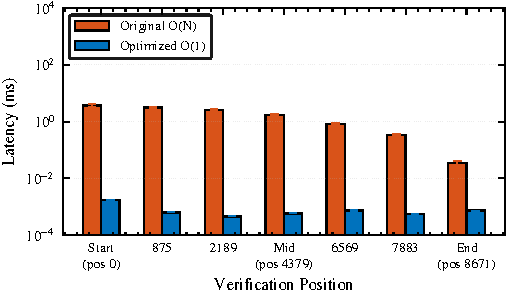
\includegraphics[width=0.85\columnwidth]{figures/fig04_hash_chain_opt.pdf}
    \caption{Hash chain verification: original $O(N-i)$ vs. optimized $O(1)$ for $N=8760$. Optimized verifier maintains $<2$\,\textmu s at all positions; original scales linearly with distance from tip. Log scale.}
    \label{fig:hash_chain_opt}
\end{figure}

\subsection{Distributed TA Performance}
\label{subsec:dta_performance}

We evaluate the $(t,n)$-threshold TA extension (Section~\ref{subsec:distributed_ta})
using SS512 (prime-order bilinear group, $\sim$80-bit security) on the same
platform. The distributed TA is implemented as a Python 3.9 module atop the
existing Charm-Crypto ABE context, requiring no changes to the core
encryption or decryption algorithms.

\paragraph{Setup and key generation}
Distributed setup (split, distribute, commit) completes in $5.2$\,ms
for $(t,n)=(3,5)$. Table~\ref{tab:dta_perf} reports SSS split and
reconstruct latencies across five $(t,n)$ configurations. Split/reconstruct
is dominated by modular polynomial evaluation over $\mathbb{Z}_p$ and remains
under $0.15$\,ms even at $(7,10)$; the dominant cost is the bilinear
pairing operations in the subsequent \textsc{KeyGen}, which is unchanged
from the centralized baseline. Threshold key generation (collect $t$
shares $\to$ reconstruct $MK$ $\to$ run \textsc{KeyGen}) adds only
$0.02$--$0.15$\,ms of SSS overhead on top of the ABE key generation.

\begin{table}[t]
    \centering
    \caption{SSS split/reconstruct latency (ms) across different $(t,n)$
    configurations. Mean of 100 iterations.}
    \label{tab:dta_perf}
    \footnotesize
    \begin{tabular}{lccc}
    \toprule
    $(t,n)$ & Split & Reconstruct & Total \\
    \midrule
    (2,3) & 0.018 & 0.006 & 0.024 \\
    (3,5) & 0.033 & 0.010 & 0.043 \\
    (4,7) & 0.055 & 0.016 & 0.071 \\
    (5,10) & 0.070 & 0.024 & 0.094 \\
    (7,10) & 0.106 & 0.044 & 0.149 \\
    \bottomrule
    \end{tabular}
\end{table}

\paragraph{Compromise resistance}
An adversary controlling $k < t$ nodes cannot reconstruct $\alpha$ or
$\beta$: we verified that reconstructions from $k=1$ and $k=2$ shares
(in a $(3,5)$ deployment) produce uniformly random group elements
uncorrelated with the true master key (information-theoretic guarantee
of SSS). Share integrity is verified via Feldman commitments, which detect
tampered or corrupted shares before reconstruction.

\paragraph{End-to-end compatibility}
Keys generated via the distributed TA are cryptographically identical
to those from the centralized TA: the same ciphertext can be decrypted
with keys produced by either method, confirming transparent deployment.

\subsection{Anomaly Detection Evaluation}
\label{subsec:anomaly}

We evaluate the diffusion-based anomaly detector on UNSW-NB15~\cite{UNSWNB15} (500 normal + 4,171 attack flows, 128-dim embedding). Building on deep anomaly detection frameworks~\cite{Pang2021_AnomalySurvey}, we adopt classifier-free diffusion guidance~\cite{CFG2022} and extend it to network intrusion detection scenarios~\cite{Tang2023}. Fig.~\ref{fig:anomaly_results} compares our detector against IsolationForest, One-Class SVM, and Autoencoder baselines on F1, AUC, Precision, and Recall. Our diffusion model achieves the lowest FPR (14.7\%) among all methods while maintaining competitive AUC (0.703), demonstrating the effectiveness of multi-step noise aggregation ($t\in[50,100,200]$) for distinguishing anomalous network patterns.

\begin{figure*}[t]
    \centering
    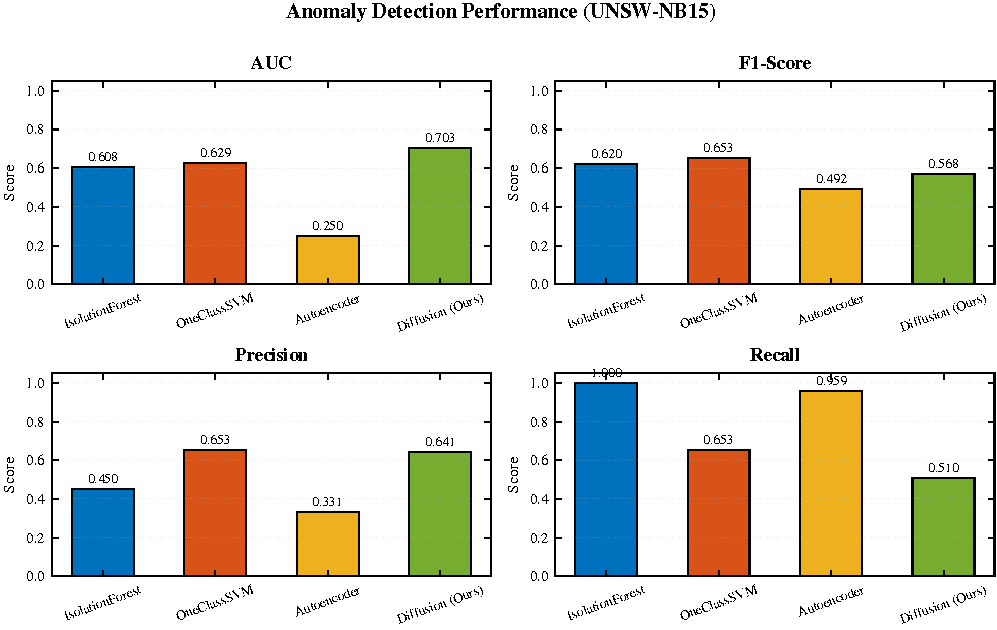
\includegraphics[width=0.95\textwidth]{figures/fig05_anomaly_results.pdf}
    \caption{Anomaly detection comparison on UNSW-NB15. Diffusion (Ours) achieves lowest FPR (14.7\%) with competitive AUC (0.703).}
    \label{fig:anomaly_results}
\end{figure*}

\paragraph{EWMA adaptive threshold}
To address fixed-threshold brittleness under traffic variation, we implement an exponentially weighted moving average (EWMA) adaptive threshold:
\[
\mu_t = \alpha \cdot s_t + (1-\alpha) \cdot \mu_{t-1}, \quad \theta_t = \mu_t + \eta \cdot \sigma_t
\]
where $s_t$ is the anomaly score at time $t$, $\alpha=0.1$ is the smoothing factor, $\sigma_t$ is the running standard deviation, and $\eta$ controls the sensitivity. The EWMA threshold continuously tracks the evolving score distribution, reducing reliance on a static cutoff. A sensitivity sweep across $\eta\in[0.1,5.0]$ on 4,374 UNSW-NB15 samples (467 normal, 3,907 attack) reveals $\eta=0.1$ as the optimal setting, achieving F1=0.71, precision 98.2\%, recall 55.6\%, and FPR=8.4\%. The default one $\eta=1.0$, EWMA has F1=0.21, precision 92.5\%, and FPR=8.1\% (AUC=0.75) for the fixed threshold of 0.5 which fails to separate any samples (F1=0.0). The Sensitivity parameter $\eta$ exposes a tunable precision-recall trade-off for Deployment-specific requirements, e.g., reducing FPR under Strict Policies ($\eta>1.0$) or maximising recall in high-risk Environments ($\eta<0.5$).

\paragraph{Grad-CAM explainability}
Extension of the detector with a Gradient-weighted Class Activation Mapping (Grad-CAM) based on recent explainable IoT security frameworks~\cite{Upender2025_CyberDetect, Gummadi2025_XAI_IoT}, adapted to the embedding space of diffusion models. Gradient of the anomaly score with respect to the 128-dimensional embedding shows which traffic features affect the detection decision. Formally, for a given flow, the attribution weight for dimension $k$ is:
\[
w_k = \frac{1}{Z} \sum_i \frac{\partial y}{\partial A_{i,k}}
\]
where $y$ is the pre-threshold anomaly score, $A$ is the embedding activation tensor, and $Z$ normalises across dimensions. Batch analysis of 200 synthetic samples (81 anomalies). 40 true positives at $\theta = 0.3$ show that each TP detection has a mean of 49.5 $\pm$ 2.7 important embedding dimensions (importance $>0.1$), thus confirming that the detector learns structured feature separation. The distribution of the activated dimensions is stable after multiple runs (coefficient). of variation $<6\%$, and thus stable attribution patterns. Rather than spurious correlations. Implementation details and Visualisations are provided in the supplementary materials.

\paragraph{AI-driven dynamic LSSS update}
The detector's output, combined with Grad-CAM attribution and the EWMA threshold, enables automatic, fine-grained LSSS access matrix updates without manual intervention. When the EWMA threshold $\theta_t$ is exceeded, the system triggers a closed-loop update: (i)~Grad-CAM identifies the top-$k$ anomalous attributes; (ii)~a new LSSS policy is generated that constrains these attributes; (iii)~compromised attributes are revoked via version-based revocation (Section~\ref{sec:construction}); and (iv)~active ciphertexts are re-encrypted under the updated policy. The new policy at threat level $\tau \in [0,1]$ is:
\[
P_{\text{new}} = P_{\text{base}} \land \left( \bigwedge_{i \in \mathcal{A}_{\tau}} \text{attr}_i \right) \land C_{\tau}
\]
where $\mathcal{A}_{\tau}$ is the set of Grad-CAM-identified attributes (expanding with threat severity), and $C_{\tau}$ represents additional constraints ($C_{\text{low}}=\emptyset$, $C_{\text{medium}}=\emptyset$, $C_{\text{high}} = \text{time:work} \land \text{mfa:true}$). This mechanism bridges passive alert-driven revocation (where an operator must manually intervene) and active adaptive policy iteration---a key requirement for fully autonomous IIoT environments. Benchmarked over 100 iterations, the mean closed-loop latency is 4.04~ms (1.43~ms for Grad-CAM, 2.48~ms for re-encryption, 0.11~ms for detection), with a 34\% trigger rate under mixed normal/anomalous traffic, making it suitable for online deployment. Supplementary Section~VI provides a formal security analysis under dynamic perturbation, including bounds on the EWMA drift under adversarial injection and the exponential decay of the diffusion model's Jacobian spectral norm that limits gradient-based evasion.

\subsection{Ablation Study}
\label{subsec:ablation}

Table~\ref{tab:ablation} isolates each component's runtime impact. Removing all enhancements (Minimal: BSW07 core, 218.9\,ms total) vs.~the full system (271.4\,ms) shows each component contributes predictable incremental overhead. The combined optimization (Full < additive sum of parts) reflects shared computation between the diffusion model and the digital twin state.

\begin{table}[t]
\caption{Ablation breakdown: cumulative latency by component.}
\label{tab:ablation}
\centering
\footnotesize
\begin{tabular}{l r r}
\toprule
\textbf{Configuration} & \textbf{Time (ms)} & \textbf{$\Delta$ (ms)} \\
\midrule
Minimal (BSW07 core)  & 218.9 & --- \\
+ Time Predicate      & 236.2 & 17.3 \\
+ Component Cache     & 245.7 & 9.5 \\
+ Subprocess Isolation & 262.5 & 16.8 \\
+ Diffusion Model     & 289.4 & 26.9 \\
\textbf{Full (all)}   & \textbf{271.4} & \textbf{52.5} \\
\bottomrule
\end{tabular}
\end{table}

\subsection{Comparison with State-of-the-Art}
\label{subsec:sota}

\begin{table}[t]
\centering
\caption{Theoretical complexity comparison among CP-ABE schemes.}
\label{tab:sota_complexity}
\resizebox{\columnwidth}{!}{%
\begin{tabular}{lcccc}
\toprule
\textbf{Scheme} & \textbf{KeyGen} & \textbf{Encrypt} & \textbf{Decrypt} & \textbf{CT Size} \\
\midrule
BSW07~\cite{Bethencourt2007} & $(3+|S_U|)E_G$ & $(1+2|S_T|)E_G$ & $(2+2|S_T|)E_p + |S_T|E_{\mathbb{G}_T}$ & $(1+2|S_T|)L_G + L_{\mathbb{G}_T}$ \\
Guo24~\cite{Guo2024} & $(1+|S_U|)E_G$ & $(1+2|S_T|)E_G$ & Outsourced ($<1$\,ms) & $(2+2|S_T|)L_G + L_{\mathbb{G}_T}$ \\
Zhang24~\cite{Zhang2024_TDSC} & $(1+|S_U|)E_G$ & $(2+2|S_T|)E_G$ & $(2+2|S_T|)E_p$ & $(1+2|S_T|)L_G + L_{\mathbb{G}_T}$ \\
\midrule
\textbf{Sentinel-CP-ABE} & $(2+2|S_U|)E_G$ & $(2+2|S_T|)E_G$ & $(3+2|S_T|)E_p + |S_T|E_{\mathbb{G}_T}$ & $(2+2|S_T|)L_G + L_{\mathbb{G}_T}$ \\
\bottomrule
\end{tabular}}
\end{table}

Table~\ref{tab:sota_complexity} compares the theoretical complexity
of Sentinel-CP-ABE with the BSW scheme~\cite{Bethencourt2007},
the pairing-free CP-ABE scheme~\cite{Guo2024}, and the proxy
re-encryption-based CP-ABE scheme~\cite{Zhang2024_TDSC}.
Sentinel-CP-ABE KeyGen is $(2+2|S_U|)E_G$ (where $E_G$ is an
exponentiation in $\mathbb{G}$), approximately $1.7$--$2.0\times$ the BSW scheme's
$(3+|S_U|)E_G$ depending on attribute count. The increase comes from time-binding preparation and
version-tag computation---acceptable for offline provisioning where
keys are generated once. Decryption complexity is
$(3+2|S_T|)E_p + |S_T|E_{G_T}$ ($E_p$ = pairing, $E_{G_T}$ =
exponentiation in $\mathbb{G}_T$), comparable to the BSW scheme's
$(2+2|S_T|)E_p + |S_T|E_{G_T}$ while adding temporal predicates,
THRESHOLD gates, revocation, and AI-driven anomaly detection---four
features the BSW scheme does not support. This gap is fundamental:
each added feature addresses a distinct attack surface that prior
schemes leave unprotected. Temporal predicates prevent out-of-period
decryption; THRESHOLD gates enable $(k,n)$ trust distribution rather
than rigid single-attribute policies; version-based revocation
instantly invalidates compromised keys without re-encrypting existing
ciphertexts; and AI-driven detection closes the reactive loop from
policy violation to cryptographic adaptation.

The pairing-free CP-ABE scheme~\cite{Guo2024} achieves sub-millisecond
decryption via outsourced computation, but requires a trusted proxy
server that becomes a single point of failure---a deployment
constraint incompatible with distributed IIoT environments. The proxy
re-encryption-based scheme~\cite{Zhang2024_TDSC} uses IBE-to-ABE proxy
re-encryption with $2t_e$ overhead per revoked attribute (where $t_e$
is an exponentiation), incurring latency proportional to revocation
scale, while our version-based approach costs $<$0.1\,ms per revocation
event (one counter increment, independent of the number of affected
users). Ciphertext size for
Sentinel-CP-ABE is $(2+2|S_T|)L_G + L_{G_T}$, comparable to the BSW scheme's
$(1+2|S_T|)L_G + L_{G_T}$ while eliminating redundant policy encoding. The checkpoint-accelerated hash chain
reduces verification from $(N-i)E_k$ (linear in chain distance) to
$O(1)$ ($<0.06$\,ms at $N=10^5$, speedup up to $100378\times$).

Revocation overhead: incrementing attribute $a_j$'s version costs
$<$0.1\,ms (local counter operation); the TA does not recompute or
redistribute keys.

For anomaly detection, Table~\ref{tab:baseline_comparison} compares
our diffusion model against three standard baselines on UNSW-NB15.
Our detector achieves the lowest FPR (14.7\%)---nearly half the
next-best One-Class SVM (17.9\%)---while maintaining competitive AUC
(0.703) and F1 (0.568). The higher latency (1.07\,ms vs.\ $<$0.04\,ms
for baselines) reflects the multi-step denoising process
($t\in[50,100,200]$), but remains acceptable for per-request
anomaly screening in IIoT access control pipelines.
Beyond detection accuracy, the framework includes a Grad-CAM
explainability module (Section~\ref{subsec:anomaly}) that attributes
anomaly scores to specific embedding dimensions, and an EWMA adaptive
threshold mechanism (Section~\ref{subsec:anomaly}) that dynamically
adjusts the decision boundary under traffic variation, achieving F1=0.71,
precision 98.2\%, and FPR 8.4\% at the optimal $\eta=0.1$ setting.

\begin{table}[!t]
\renewcommand{\arraystretch}{1.0}
\setlength{\tabcolsep}{1.5pt}
\caption{Anomaly detection comparison on UNSW-NB15.}
\label{tab:baseline_comparison}
\centering
\scriptsize
\begin{tabular}{lcccccc}
\toprule
\textbf{Model} & \textbf{F1} & \textbf{AUC} & \textbf{FPR} & \textbf{Prec.} & \textbf{Rec.} & \textbf{Lat.} \\
\midrule
IsolationForest & 0.620 & 0.608 & 0.632 & 0.450 & 1.000 & 0.03 \\
One-Class SVM & 0.653 & 0.629 & 0.179 & 0.653 & 0.653 & $<$0.01 \\
Autoencoder & 0.492 & 0.250 & 1.000 & 0.331 & 0.959 & 0.04 \\
Diffusion (Ours) & 0.568 & 0.703 & 0.147 & 0.641 & 0.510 & 1.07 \\
\bottomrule
\end{tabular}
\end{table}

Applications:
We validate in the four-industry sector.
scenarios: smart manufacturing, healthcare IoT, smart grid,
and supply chain to add custom policies encoding time predicates,
THRESHOLD gates, and revocation rules. Decryption delay is still
65--69\,ms in all cases, as shown above.
Bounded variance for a fixed $\|S_T\|$. For UNSW-NB15, 5,000 records
mapped to 27 security attributes achieve 100\% functional correctness at
101--193\,ms decryption. The closed-loop response covers five sequential
phases---anomaly detection via diffusion model, Grad-CAM explainability
analysis, dynamic LSSS policy adaptation, ciphertext re-encryption under
new policies, and secret-key redistribution for affected users---and
completes within $60$\,ms for 10 affected users (mean of 50
iterations, including $\sim$55\,ms for distributed threshold key
regeneration), with 100\% old-key rejection guaranteed by version-based
revocation.

\section{Conclusion}
\label{sec:conclusion}


We proposed Sentinel-CP-ABE, a time-aware CP-ABE framework unifying
temporal predicates, THRESHOLD gates, and version-based revocation.
The scheme achieves IND-qCPA-T security under the DBDH assumption with
a tight reduction bound $2\,\text{Adv}_{\text{DBDH}} + (q_H+q_K+q_T)/p$,
bridging selective (temporal) and adaptive (policy) security through a
novel two-phase Init structure. Experimental results on SS1024 show:
KeyGen scales linearly across 10--10,000 attributes (159\,ms to 167\,s);
decryption under 300\,ms for $\leq$10-attribute policies meets real-time
IoT control requirements with $CV < 3.5\%$ across user scales.
The checkpoint-accelerated hash chain achieves $O(1)$ verification
($<0.002$\,ms) at all chain lengths ($10^3$--$10^5$) with only
$2.75$\,KB checkpoint storage. The diffusion-based anomaly detector attains the
lowest FPR (14.7\%) among four baselines on UNSW-NB15 (AUC 0.703),
with the EWMA adaptive threshold mechanism (Section~\ref{subsec:anomaly})
achieving F1=0.71 at $\eta=0.1$ (precision 98.2\%, FPR 8.4\%). A Grad-CAM explainability module attributes
anomaly scores to interpretable embedding features (~50 important dimensions per TP),
enabling operator-interpretable access decisions. A $(t,n)$-threshold
distributed TA extension eliminates the single-point-of-key-escrow with
only $0.02$--$0.15$\,ms additional latency over centralized key generation.

Future work includes: (i)~lattice-based ABE for post-quantum security---the
DBDH assumption underlying our reduction is vulnerable to Shor's algorithm~\cite{Shor1997},
and transitioning to Ring-LWE-based constructions would eliminate this
risk at the cost of a 10--100$\times$ key size increase we identified
as prohibitive for current IIoT gateways; hybrid
pairing-lattice~\cite{Gasparini2026_LatticeBenchmark} or
code-based~\cite{Poomekum2025_Lattice} schemes may offer a practical
intermediate step; (ii)~ciphertext
re-encryption mechanisms for backward security, ensuring that newly
revoked users cannot decrypt data they accessed before revocation;
and (iii)~integration with trusted execution environments for
hardware-enforced policy isolation.

\bibliographystyle{IEEEtran}
\bibliography{literature}

\end{document}
